\documentclass[12pt,a4paper]{report}
\usepackage[utf8]{inputenc}
\usepackage{amsmath}
\usepackage{algorithm}
\usepackage{algpseudocode}
\usepackage{amssymb}
\usepackage{graphicx}
\usepackage{geometry}
\usepackage[hidelinks]{hyperref}  % For clickable references
\usepackage[capitalise]{cleveref}  % For intelligent cross-referencing
\usepackage[english]{babel}

\usepackage{makecell}
\usepackage{caption}
\usepackage{array}
\usepackage{listings}
\usepackage{titlesec}
\usepackage{hyperref}
\hypersetup{
	colorlinks=true,
	linkcolor=black,
	filecolor=black,      
	urlcolor=cyan,
	citecolor=black
}

\graphicspath{{C:/Users/frabb/OneDrive - Cal Poly/Documents (Cloud)/0 CALPOLY/000Thesis/Chapters/Images/}}

\geometry{
	top=1in,
	bottom=1in,
	left=1.5in,
	right=1in
}

% Remove space before equations only
\makeatletter
\g@addto@macro\normalsize{%
	\setlength\abovedisplayskip{-10pt}
	\setlength\abovedisplayshortskip{-10pt}
}
\makeatother

% Updated list settings
\usepackage{enumitem}
\setlist[itemize]{nosep, leftmargin=*}
\setlist[enumerate]{nosep, leftmargin=*}

% Remove space before lists
\usepackage{etoolbox}
\BeforeBeginEnvironment{itemize}{\vspace{-\baselineskip}}
\BeforeBeginEnvironment{enumerate}{\vspace{-\baselineskip}}

\setlength{\parskip}{\baselineskip}
\titlespacing*{\section}{0pt}{0pt}{0pt}
\titlespacing*{\section}{0pt}{0pt}{-10pt}
\titlespacing*{\subsection}{0pt}{0pt}{-10pt}

\captionsetup[table]{skip=0pt}

\usepackage{xcolor}

\definecolor{codegreen}{rgb}{0,0.6,0}
\definecolor{codegray}{rgb}{0.5,0.5,0.5}
\definecolor{codepurple}{rgb}{0.58,0,0.82}
\definecolor{backcolour}{rgb}{0.95,0.95,0.92}

\lstdefinestyle{mystyle}{
	backgroundcolor=\color{backcolour},   
	commentstyle=\color{codegreen},
	keywordstyle=\color{magenta},
	numberstyle=\tiny\color{codegray},
	stringstyle=\color{codepurple},
	basicstyle=\ttfamily\footnotesize,
	breakatwhitespace=false,         
	breaklines=true,                 
	captionpos=b,                    
	keepspaces=true,                 
	numbers=left,                    
	numbersep=5pt,                  
	showspaces=false,                
	showstringspaces=false,
	showtabs=false,
	tabsize=2
}

\lstset{style=mystyle}

\title{Tutorial}
\author{Jakob Frabosilio}
\date{\today}
\setcounter{chapter}{3}
\begin{document}

\chapter{Absolute Orientation and Dead Reckoning} \label{chap:4c}
As seen in Chapter \ref{chap:3c}, having an accurate orientation estimate of the iSBL array is crucial for getting the position estimate of the array. Without it, the system is unable to transform the relative position estimate to the global/test frame. This chapter details how that orientation estimate is formed. Additionally, the concept of “dead reckoning” is introduced and its integration into the iSBL-SF algorithm is explained.

The first section of this chapter covers the various methods of orientation estimation, compares them to the method chosen for this thesis, and explores some implementations in related works. Next, the choice of IMU for this thesis is discussed, and its software implementation (interfacing with STM32, initialization, and calibration) is explained. The chosen orientation estimation method for this thesis, the Madgwick filter, receives its own section: it covers the theory of the Madgwick filter (including an explanation of quaternions) and the code implementation of the filter. Dead reckoning is introduced and its software execution is shown. Finally, both the orientation estimation system and the dead reckoning system are validated experimentally.

\section{Background and Previous Works} \label{sec:4s1}
This section is split into two subsections: the first covers the history of orientation estimation and the development of MEMS IMUs; the second compares different sensor fusion algorithms for converting MEMS IMU readings into an absolute orientation estimate, and mentions some implementations of these filters.

\subsection{Introduction to IMUs and Orientation Estimation} \label{ssec:4s1s1}
Estimating the absolute orientation of a system (generally, the orientation relative to the global frame) is a common problem in both robotics and marine navigation. Early ocean navigators, such as the Phoenecians and the Polynesians, used celestial and environmental navigation techniques to sail from place to place. It took nearly 2000 years of development for compasses to become reliable and commonplace in ships, and another 500 years before gyrocompasses (electrically-powered gyroscopes that maintain a certain orientation and can be aligned to point towards north) were invented \cite{shipscompass}. In the past 100 years, orientation and heading estimation technology has advanced at an incredible rate; mechanical gyroscopes have improved and can be shrunk down to fit inside of commercial planes, spacecraft, and missile systems \cite{v2missile}. While quite costly, modern mechanical and ring-laser gyroscopes can provide extremely accurate orientation estimates for mission-critical systems \cite{shipscompass}.

\begin{figure}[htbp]
	\centering
	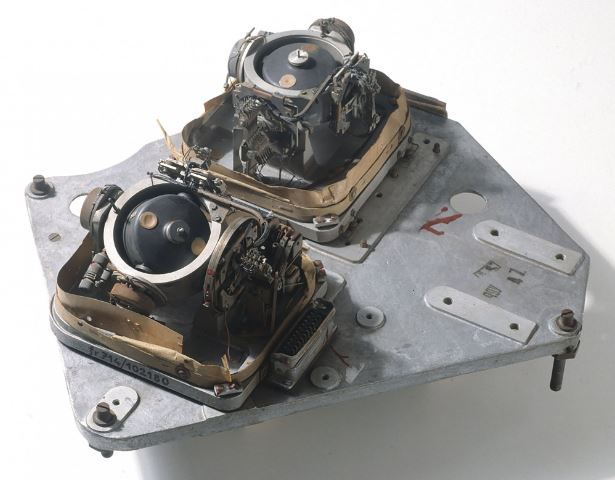
\includegraphics[width=0.65\textwidth]{v2gyro}
	\caption{V2 missile gyroscope \cite{v2missile}}
	\label{fig:v2gyro}
\end{figure}

With the development of semiconductor technology, a new inertial navigation technology was created: MEMS IMUs. Micro-electro-mechanical systems (MEMS) are small devices made using semiconductor-fabrication technology. Inertial measurement units (IMUs) are systems that combine accelerometers (which measure linear acceleration and gravity), gyroscopes (which measure angular velocity), and sometimes magnetometers (which measure magnetic field strength, like that of the Earth’s). IMUs are used in many modern aircraft, boat, and vehicle systems for attitude and heading reference. These IMU components can be manufactured as MEMS devices and are often packaged as integrated circuits, which can be as small as a ladybug (see Figure \ref{fig:bno055}) \cite{imuadvnav}.

\begin{figure}[htbp]
	\centering
	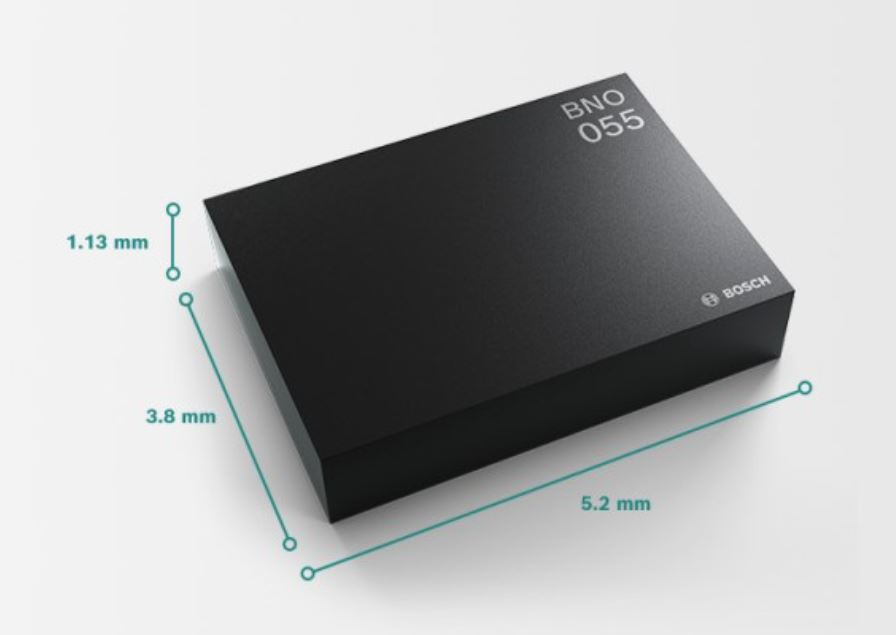
\includegraphics[width=.6\textwidth]{bno055}
	\caption{BNO055 IMU integrated circuit chip size \cite{bno055}}
	\label{fig:bno055}
\end{figure}

These MEMS IMUs are not as accurate as their macro-sized equivalents, but have considerable benefits over them. First, they can be orders of magnitude less expensive than traditional IMUs; the IMU purchased for this thesis cost \$25, while a non-MEMS IMU would often be in the thousands of dollars. They are also much easier to set up and maintain, not having any macro-scale moving components. Lastly, they are commonly used in modern, small-scale robotics systems and have gained a large consumer market. MEMS IMUs come in different performance levels with varying degrees of accuracy and applications (hobbyist and consumer, industrial, high-end tactical), providing a good range of options for different price points and needs \cite{imuadvnav}. See Figure \ref{fig:imucomp} for a comparison of these performance levels.

\begin{figure}[htbp]
	\centering
	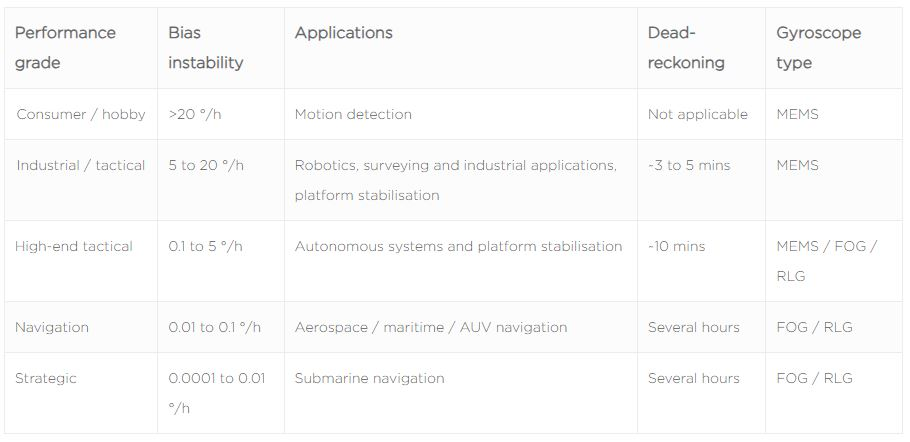
\includegraphics[width=\textwidth]{imucomp}
	\caption{IMU performance level comparison \cite{imuadvnav}}
	\label{fig:imucomp}
\end{figure}

The components of MEMS IMUs do not automatically generate an orientation estimate; an algorithm must be applied to convert the raw acceleration, angular velocity, and (sometimes) magnetic field strength readings into a usable orientation estimate relative to the global frame. This method, combining measurements from multiple unique sensors to obtain an estimate of some parameter (like orientation) is called sensor fusion. High-end MEMS IMUs tend to perform this sensor fusion for the user, while most low-cost MEMS IMUs (like the one in this thesis) require the user to compute the orientation estimation themselves. Some low-cost MEMS IMUs like the Bosch BNO055 do come with sensor fusion algorithms built in \cite{bno055}, but these techniques are generally proprietary and this approach is less common for hobbyist-level MEMS IMUs.

For the remainder of this paper, it will be assumed that the IMUs used will include magnetometers, and that they are MEMS  IMUs. An IMU that contains a magnetometer may be called a MARG (magnetic, angular rate, and gravity) \cite{madgwick}, a MIMU (magnetic inertial measurement unit) \cite{sfcomp}, or just an IMU \cite{imuadvnav}. For simplicity, this thesis will use this last approach. Whenever IMU is mentioned in this paper, it should be assumed that it contains a 3-axis accelerometer, gyroscope, and magnetometer.

\subsection{IMU Sensor Fusion Algorithms} \label{ssec:4s1s2}
The basic idea of any IMU sensor fusion algorithm is combining the long-term accuracy of accelerometers and magnetometers with the short-term accuracy of gyroscopes. When stationary, 3-axis accelerometers can detect the gravitational field of Earth and the strength along each axis to determine where “down” is. Similarly, when stationary and isolated from other magnetic fields, a 3-axis magnetometer can detect the magnetic field of Earth and use it to determine where magnetic north is; it should be noted that “true north” and “magnetic north” do not point in the same direction and that the meaning of “down” can vary at different longitudes and latitudes, two things that must be taken into consideration for advanced / “mission-critical” systems \cite{imuadvnav}. 

In an ideal world, these two sensors could provide the 3D orientation relative to the Earth frame for any object that they are attached to. However, real-world systems are often not perfectly stationary, and robotic systems in particular tend to have stray magnetic fields produced by large electric motors and other circuitry in the system. A gyroscope can be used to account for short-term movements by measuring the angular velocity of the system; these measurements are primarily used when the system is rotating or accelerating, where the accelerometer and magnetometer readings become noisy. A gyroscope alone cannot be used for accurate orientation estimation; even if the initial orientation of the system was known perfectly, any miniscule error would propagate over time and produce a wildly-drifting orientation estimate. This problem will return in Section \ref{sec:4s5}.

For low-cost MEMS IMUs, there are a few sensor fusion algorithms that are commonly used. For these examples, the orientation will be represented by the quaternion \(\mathbf{q}\) - quaternion representation will be discussed in Section \ref{ssec:4s4s1}. The most basic is a complementary filter, where a weighted average combines the orientation estimate given by the accelerometer and magnetometer with the change in orientation given by the gyroscope \cite{sfcomp}. An example of a complementary filter is shown below in Equation \ref{eq:compf}.

\begin{equation} \label{eq:compf}
	\mathbf{q}_n = (1 - \gamma) \mathbf{q}_{acc/mag} + \gamma (\mathbf{q}_{n-1} + \Delta t \times \mathbf{q}_{gyro})
\end{equation}

A Mahony filter, invented by Robert Mahony et al. in 2010, attempts to minimize the error between the gyroscope orientation estimate and the accelerometer/magnetometer orientation estimate. It implements a proportional and integral feedback controller to minimize this error, and uses two tunable gains \cite{mahony}. Figure \ref{fig:mahony} shows the algorithm for a Mahony filter.

\begin{figure}[htbp]
	\centering
	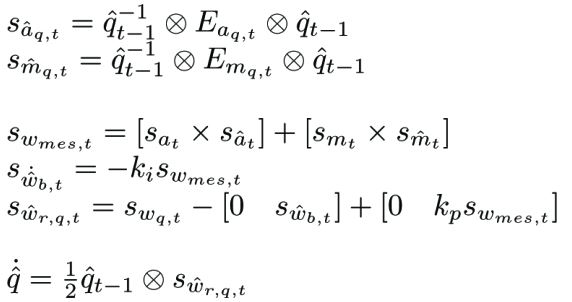
\includegraphics[width=0.6\textwidth]{mahony}
	\caption{Mahony filter algorithm \cite{ekfmadmah}}
	\label{fig:mahony}
\end{figure}

A Madgwick filter, invented by Sebastian Madgwick in 2010, is a gradient descent-based orientation estimation filter. It formulates the problem as an optimization task, attempting to minimize the error between the current (overall) orientation estimate and the accelerometer/magnetometer orientation estimate. It compensates for gyroscope and magnetometer bias/drift and only uses one tuning parameter \cite{madgwick}. Section \ref{ssec:4s4s2} covers the theory in more depth.

An extended Kalman filter is possibly the most common algorithm used for orientation estimation of IMUs. Kalman filters are explained in depth in Chapter \ref{chap:5c}; an extended Kalman filter is a modified version that works with non-linear systems (standard Kalman filters assume a linear state-space model). One particular implementation of a USBL system, mentioned in Section \ref{ssec:3s1s3}, used an extended Kalman filter to merge raw IMU data with acoustic position estimates. This approach by Morgado, Oliveira, and Silvestre from the Technical University of Lisbon, Portugal gave very promising results - close to a 15\% improvement level compared to loosely-coupled acoustic positioning systems \cite{tightekf} (like the one in this thesis). This tightly-coupled approach was considered for this thesis, but was deemed out-of-scope. For future implementations, a more tightly-coupled approach would be recommended.

The Mahony, Madgwick, and extended Kalman filters are very comparable in accuracy; generally, extended Kalman filters are the most accurate out of the three, but come at a relatively high computational cost compared to Mahony and Madgwick filters \cite{madgwick} \cite{sfcomp}. These two filters are also specifically formulated and optimized to work with IMUs, while the extended Kalman filter is a more general framework. See Figure \ref{fig:threecomp} for an accuracy comparison of the three filters in a quadrotor implementation, and the associated time for 6041 filter updates of each algorithm in Figure \ref{fig:threecomptime} \cite{ekfmadmah}. See Figure \ref{fig:eulermadg} for the orientation estimate accuracy of a Madgwick filter, versus Figure \ref{fig:eulermaho} for the accuracy of a Mahony filter, both in a pedestrian gait-measuring implementation \cite{sfcomp}.

\begin{figure}[htbp]
	\centering
	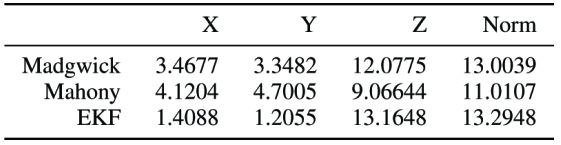
\includegraphics[width=0.5\textwidth]{threecomp}
	\caption{Accuracy comparison for Madgwick, Mahony, and extended Kalman filters in quadrotor implementation \cite{ekfmadmah}}
	\label{fig:threecomp}
\end{figure}

\begin{figure}[htbp]
	\centering
	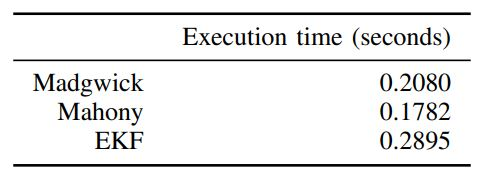
\includegraphics[width=0.5\textwidth]{threecomptime}
	\caption{Computation time comparison for 6401 filter updates \cite{ekfmadmah}}
	\label{fig:threecomptime}
\end{figure}

\begin{figure}[htbp]
	\centering
	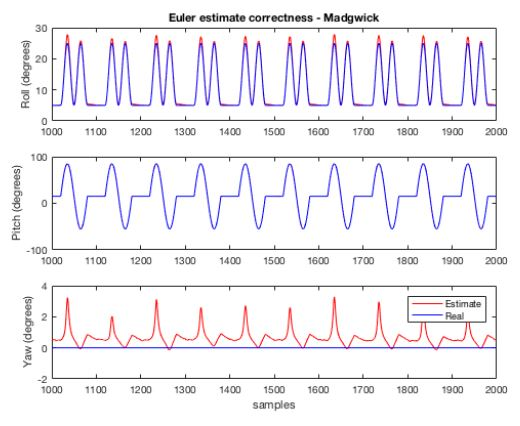
\includegraphics[width=0.75\textwidth]{eulermadg}
	\caption{Madgwick filter orientation accuracy, pedestrian implementation \cite{sfcomp}}
	\label{fig:eulermadg}
\end{figure}

\begin{figure}[htbp]
	\centering
	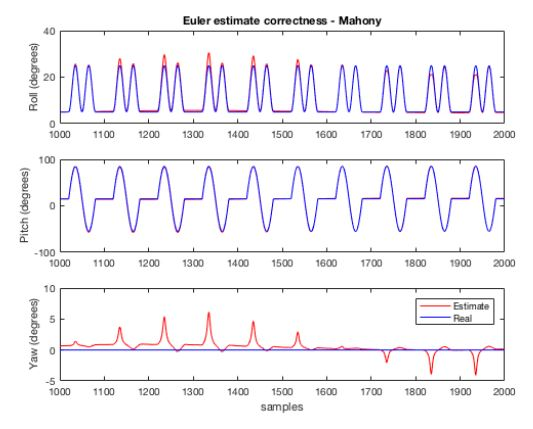
\includegraphics[width=0.8\textwidth]{eulermaho}
	\caption{Mahony filter orientation accuracy, pedestrian implementation  \cite{sfcomp}}
	\label{fig:eulermaho}
\end{figure}

For this implementation, a Madgwick filter was chosen. It provides a good orientation estimate and has a low computational cost, only has one filter gain to tune, is specifically optimized to work with IMUs, and the original Madgwick paper contains a C code implementation of the filter \cite{madgwick}. More specifics on this filter and its implementation can be found in Section \ref{sec:4s4}.

\pagebreak

\section{IMU Selection and Interfacing} \label{sec:4s2}
The selection of the MEMS IMU was critical to obtaining an accurate orientation estimate. A MEMS IMU was chosen over other orientation sensors due to its low cost, easy interfacing, and widespread use throughout hobbyist and commercial applications (see Section \ref{ssec:4s1s1}). However, throughout testing, the IMU was by far the most inaccurate component; for a full underwater implementation, a more reliable and accurate IMU (either high-end MEMS or low-end fiber optic gyroscope) would greatly improve positional accuracy. 

There are many MEMS IMUs available for consumers and hobbyists; the most common are the MPU-6050 and the MPU-9050 \cite{mpu6050}. These IMUs have open-source libraries written in multiple embedded programming languages and are featured in many hobby projects, but tend to be fairly inaccurate compared to other offerings; additionally, many clones of the sensor exist and it is difficult to identify genuine sensors when buying from third-party retailers. For example, out of six MPU-6050s purchased for the Fo-SHIP in Chapter \ref{chap:2c}, only one gave accurate accelerometer information. Other IMUs like the Bosch BNO055 are generally more reliable and provide more accurate measurements; the BNO055 even has a sensor fusion algorithm built in to the chip \cite{bno055}. While a good step up from the MPU-9050, its sensor fusion algorithm is closed-source, and couldn't be modified for a particular use case. 

After much research, a two-part IMU was chosen for its low cost, high accuracy, and availability of pre-written C drivers: the STMicroelectronics LSM6DSOX 3-axis accelerometer and gyroscope and LIS3MDL 3-axis magnetometer. Both ICs are available on a single development board from Adafruit (an online electronics retailer) with documentation and examples for the development board readily available \cite{adafruit}. Both the LSM6DSOX and LIS3MDL are automotive-rated, have low power consumption, and have relatively high sensitivities and data rates \cite{lsm6dsox} \cite{lis3mdl}. Both communicate using the I\textsuperscript{2}C protocol, which makes interfacing with the STM32 microcontroller much easier. For a full underwater implementation, a different communications protocol may be desired; the current I\textsuperscript{2}C implementation requires a request to be sent from the microcontroller to either sensor before sensor data is sent, which reduces the maximum data transmission rate of all three IMU sensors.

\begin{figure}[htbp]
	\centering
	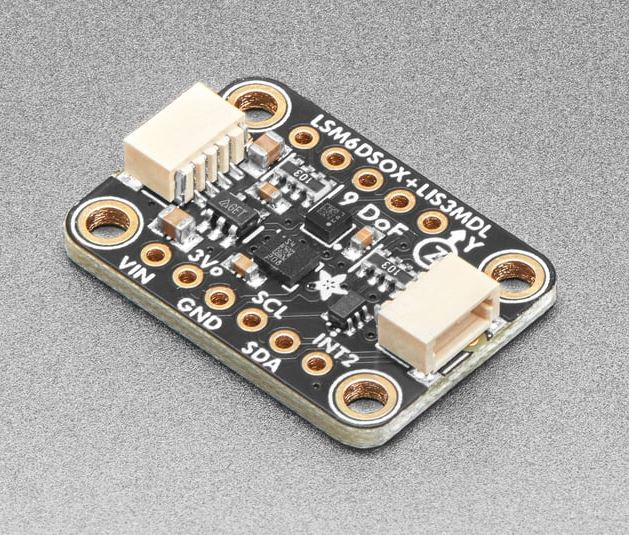
\includegraphics[width=0.45\textwidth]{theimu}
	\caption{LSM6DSOX + LIS3MDL IMU \cite{adafruit}}
	\label{fig:theimu}
\end{figure}

An important note should be made of the IMU development board’s orientation relative to the iSBL array. Figure \ref{fig:isblnaked} in Section \ref{sec:3s2} shows the coordinate frame of the iSBL array, and Figure \ref{fig:isblfront} in Section \ref{sec:3s5} shows the fully-assembled iSBL array; close inspection shows that the IMU is mounted at a 45° angle relative to the y-axis. This is due to poor planning - the original design had the iSBL array rotated 45° about the x-axis, with the microphone arms forming a “+” (instead of the current “x”). In this configuration, the Fo-SHIP was unable to pitch forward due to the bottom microphone interfering with the lower platforms. So, to get the IMU data in the correct coordinate frame, a transformation must be applied; this transformation is covered in more detail below. Figure \ref{fig:imucoord} shows the IMU coordinate frame overlaid on the iSBL array coordinate frame.

\begin{figure}[htbp]
	\centering
	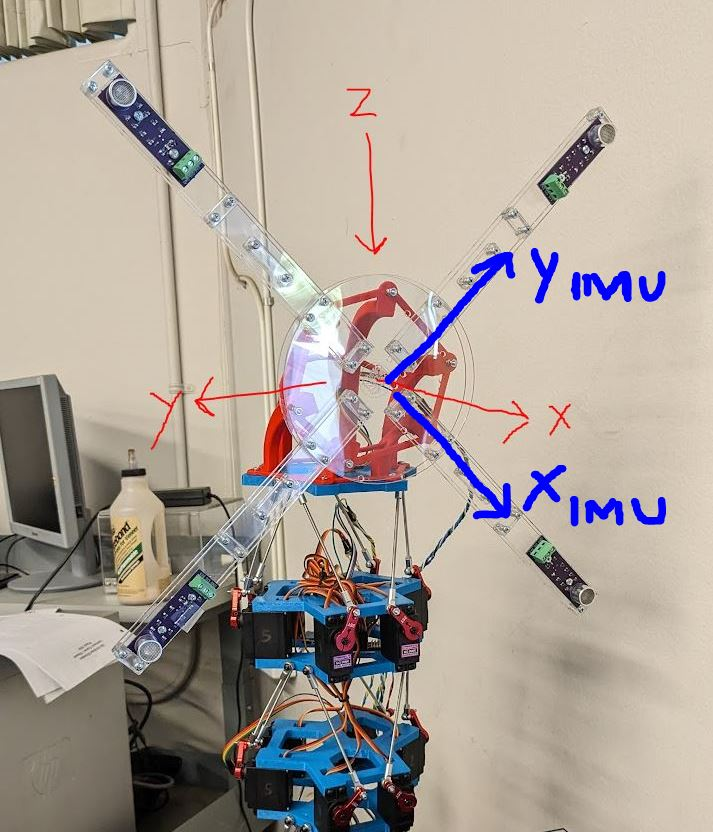
\includegraphics[width=0.7\textwidth]{imucoord}
	\caption{Raw IMU coordinate frame (blue) and iSBL array coordinate frame (red)}
	\label{fig:imucoord}
\end{figure}

Interfacing with the IMU involves communicating with both ICs independently; thankfully, STMicroelectronics provides platform-independent drivers for both sensors, along with example implementations \cite{lis3mdl_st} \cite{lsm6dsox_st}. The interfacing functions described below are modified versions of the provided drivers. Each sensor requires four unique functions to interface using I\textsuperscript{2}C. Additionally, each sensor has its own I\textsuperscript{2}C address, even though they are on the same development board.

There are four functions used for interfacing with the LSM6DSOX:
\begin{itemize}[noitemsep,topsep=0pt,]
	\item \verb|lsm6dsox_write()|
	\item \verb|lsm6dsox_read()|
	\item \verb|lsm6dsox_read_data_drdy()|
	\item \verb|lsm6dsox_read_data_drdy_handler()|
\end{itemize}

The first two functions are simple wrappers for the STM32 I\textsuperscript{2}C read/write functions. Because the drivers provided by STMicroelectronics are platform-independent, wrappers are used for the hardware-specific functions. These functions are where the I\textsuperscript{2}C address of the LSM6DSOX is declared.

The next function, \verb|lsm6dsox_read_data_drdy()|, is the initialization function for the LSM6DSOX. In this function, the data rates, accelerometer and gyroscope scales, and data transmission settings are declared. Both the accelerometer and gyroscope are set to update at 208Hz; anything above this was too fast for the STM32 microcontroller, since it is also running the acoustic position estimation code (and updating the Madgwick filter every time the IMU sends data). 

The last function, \verb|lsm6dsox_read_data_drdy_handler()|, reads the current acceleration and angular velocity data from the LSM6DSOX. The acceleration data is converted from mg (milli-g’s) to g (1g = 32.174 ft/s\textsuperscript{2}), and the angular velocity data is converted from mdps (milli-degrees per second) to dps. As stated in a previous paragraph, the coordinate frame of the IMU needs to be converted to the iSBL array coordinate frame. This is achieved using a linear combination for the y- and z-axes of the array frame, and a simple axis swap for the x-axis. The raw accelerometer data is saved in a global list \verb|acceleration_g[]|, and the raw gyroscope data is saved in a global list \verb|angular_rate_dps[]|. Finally, if the gyroscope has been calibrated, calibration biases are subtracted from each element of \verb|angular_rate_dps[]|.

\begin{lstlisting}[language=C++]
void lsm6dsox_read_data_drdy_handler(void)
{
	uint8_t reg;
	
	/* Read output only if new xl value is available */
	lsm6dsox_xl_flag_data_ready_get(&dev_ctx, &reg);
	
	if (reg) {
		/* Read acceleration field data */
		memset(data_raw_acceleration, 0x00, 3 * sizeof(int16_t));
		lsm6dsox_acceleration_raw_get(&dev_ctx,data_raw_acceleration); 
		// Note: acceleration data is negative by default
		// Z-axis reading to X
		acceleration_g[0] = -lsm6dsox_from_fs4_to_mg(data_raw_acceleration[2]) / 1000.0; 
		
		// Combination of X and Y to Y
		acceleration_g[1] = 0.7071 * (lsm6dsox_from_fs4_to_mg(data_raw_acceleration[0]) / 1000.0 + lsm6dsox_from_fs4_to_mg(data_raw_acceleration[1]) / 1000.0);    
		
		// Combination of X and Y to Z
		acceleration_g[2] = 0.7071 * (-lsm6dsox_from_fs4_to_mg(data_raw_acceleration[0]) / 1000.0 + lsm6dsox_from_fs4_to_mg(data_raw_acceleration[1]) / 1000.0);   
	}
	
	lsm6dsox_gy_flag_data_ready_get(&dev_ctx, &reg);
	
	if (reg) {
		/* Read angular rate field data */
		memset(data_raw_angular_rate, 0x00, 3 * sizeof(int16_t));
		lsm6dsox_angular_rate_raw_get(&dev_ctx,data_raw_angular_rate);
		
		// Z-axis reading to X
		angular_rate_dps[0] = lsm6dsox_from_fs1000_to_mdps(data_raw_angular_rate[2]) / 1000.0;
		
		// Combination of X and Y to Y          
		angular_rate_dps[1] = 0.7071 * (-lsm6dsox_from_fs1000_to_mdps(data_raw_angular_rate[0]) / 1000.0 - lsm6dsox_from_fs1000_to_mdps(data_raw_angular_rate[1]) / 1000.0);
		
		// Combination of X and Y to Z
		angular_rate_dps[2] = 0.7071 * (lsm6dsox_from_fs1000_to_mdps(data_raw_angular_rate[0]) / 1000.0 - lsm6dsox_from_fs1000_to_mdps(data_raw_angular_rate[1]) / 1000.0);
		
		// Apply gyroscope calibration only if it has already been calibrated
		if (imu_calibrated){
			angular_rate_dps[0] += g_cal[0];
			angular_rate_dps[1] += g_cal[1];
			angular_rate_dps[2] += g_cal[2];
		}
	}
}
\end{lstlisting}

The LIS3MDL has four functions to get magnetic field strength readings:
\begin{itemize}[noitemsep,topsep=0pt,]
	\item \verb|lis3mdl_write()|
	\item \verb|lis3mdl_read()|
	\item \verb|lis3mdl_read_data_drdy()|
	\item \verb|lis3mdl_read_data_drdy_handler()|
\end{itemize}

The first two functions, \verb|lis3mdl_write()| and \verb|lis3mdl_read()|, are nearly identical to their LSM6DSOX counterparts; the only difference is the I\textsuperscript{2}C address.

The third function, \verb|lis3mdl_read_data_drdy()|, is the initialization function for the LIS3MDL. It is similar to its LSM6DSOX counterpart, but uses a different sampling rate of 80Hz - the maximum sampling rate for the magnetometer. 

The final function, \verb|lis3mdl_read_data_drdy_handler()|, reads the magnetic field strength data from the LIS3MDL. Both the LIS3MDL and LSM6DSOX share the same coordinate frame, so the transform to the iSBL array coordinate frame is the same as in the \verb|lsm6dsox_read_data_drdy_handler()| function.

When the LSM6DSOX updates every 4.81ms, the INT2 pin on the development board is pulsed. This pin is connected to a GPIO pin on the STM32 which is set up in interrupt mode. When the interrupt is triggered (and if the IMU has been set up), the STM32 stops whatever task it is running and executes the following:

\begin{lstlisting}[language=C++]
void HAL_GPIO_EXTI_Callback(uint16_t GPIO_Pin)
{
	if (imu_rdy){
		if (GPIO_Pin == GPIO_PIN_8)
		{
			lis3mdl_read_data_drdy_handler();
			lsm6dsox_read_data_drdy_handler();
			data_rdy = 1;
			if (imu_calibrated && !recording){
				update_filter();
			}
		}
	}
}
\end{lstlisting}

Note that since the accelerometer and gyroscope update rate is more than double the magnetometer update rate, the same magnetometer measurements get used multiple times. This is a necessary simplification, as the current Madgwick filter implementation requires all nine measurements (3-axis for each sensor) to perform an update. If the system were switched to a tightly-coupled extended Kalman filter as mentioned in Section \ref{ssec:4s1s2}, it would be possible (and preferred) to update the measurements separately.

\section{IMU Setup, Calibration, and Initialization} \label{sec:4s3}
The IMU is set up and calibrated in the initialization state of the STM32 program, and an initial orientation is formed after 10,000 measurements. The set-up and calibration are performed by one function, \verb|init_imu()|.

\begin{lstlisting}[language=C++]
void init_imu(void){
	lis3mdl_read_data_drdy();
	lsm6dsox_read_data_drdy();
	lis3mdl_read_data_drdy_handler();
	lsm6dsox_read_data_drdy_handler();
	gyro_calibration(g_cal, 256);
}
\end{lstlisting}

First, the initialization functions for the LIS3MDL and LSM6DSOX are called. At the end of the \verb|lsm6dsox_read_data_drdy()| function, a global flag \verb|imu_rdy| is set to \verb|1|. Before this step, the IMU is not configured for the proper data rates or sensitivities, so it should not be read from. Then, the data reading functions for each IC are called once; this triggers both sensors to start updating their measurements at their set data rates.

Calibrating a MEMS IMU is one of the most important steps in getting accurate data \cite{imuadvnav}. The three sensors on the IMU have known sources of error that can be mitigated: a gyroscope at rest should not measure any angular velocity; an accelerometer at rest should only measure gravity \cite{imucal}; and a magnetometer rotated about all its axes should measure an equal, non-skewed magnetic field \cite{magcal}.

To calibrate the gyroscope, the IMU is held at rest and multiple (256, in this implementation) measurements are taken. Assuming that the IMU is truly at rest, the readings for each axis should average to zero; noise from the environment and sensor will produce readings that are not perfectly zero, but taking an average of a large number of samples mitigates this noise. However, MEMS gyroscopes tend to have some constant offset (called a bias) when at rest. This bias can be measured and subtracted from subsequent readings after calibration is complete. Note that the calibration function is a blocking function in this implementation and relies on the LSM6DSOX triggering interrupts on the INT2 pin.

\begin{lstlisting}[language=C++]
void gyro_calibration(float g_cal[3], int num_iter){
	for (int i = 0; i < num_iter; i++){
		while (!data_rdy);
		g_cal[0] -= angular_rate_dps[0];
		g_cal[1] -= angular_rate_dps[1];
		g_cal[2] -= angular_rate_dps[2];
		data_rdy = 0;
	}
	g_cal[0] /= (float)num_iter;
	g_cal[1] /= (float)num_iter;
	g_cal[2] /= (float)num_iter;
	imu_calibrated = 1;
}
\end{lstlisting}

Many of the calibration models for IMUs assume a linear model for measurements, like that in Equation \ref{eq:compf}. This assumes that the true value of the measurement can be described by the raw measurement \verb|x| times a gain \verb|K| plus a bias \verb|b|. Often, these are formulated with measurements and bias as vectors and gains as matrices \cite{imucal}.

\begin{equation} \label{eq:compf}
	\mathbf{x}_{calibrated} = \mathbf{K}\mathbf{x}_{raw} + \mathbf{b}
\end{equation}

In a complete system, each sensor should be calibrated according to this model. For this implementation, only the gyroscope is calibrated and only a bias term is considered. Measuring the gain matrix for the gyroscope is not possible without external equipment.

Calibrating the accelerometer and magnetometer requires rotating the IMU in a controlled manner. The Fo-SHIP may appear capable of doing this, but calibration routines require placing the IMU level on its six faces (for the accelerometer) and rotating it around in every possible orientation (for the magnetometer). This motion is not possible with the Fo-SHIP, and the IMU has been permanently affixed to the iSBL array with adhesive prior to calibration being considered. With better planning, it would have been possible to calibrate the IMU before attaching it to the array. This approach is highly recommended for future implementations, and calibration routines for the accelerometer \cite{imucal} and magnetometer \cite{magcal} are available in the references of this thesis.

The final step in the initialization of the IMU is measuring an initial orientation estimate. As mentioned in Section \ref{ssec:3s9s1}, the yaw component of the initial orientation must be removed to transform the acoustic position estimates from the global frame to the test frame. Before the first Madgwick filter update, the orientation estimate is simply the unit quaternion \(\mathbf{q}_0 = [1, 0, 0, 0]\). This estimate is slowly affected by new IMU measurements; it doesn’t automatically move to the true orientation of the platform. After a set number of filter updates (10,000, in this implementation), the Madgwick filter will have converged on a good orientation estimate - the quaternion is then saved and the initial yaw is extracted. The number of iterations required depends on the filter gain \verb|beta|, the update frequency of the IMU, and the initial orientation relative to the global frame.

\begin{lstlisting}[language=C++]
void update_filter(void)
	...
	// if the filter has converged, set the initial quaternion
	if (imu_i == -1){
		initQuat.w = q0;
		initQuat.x = -q1;
		initQuat.y = -q2;
		initQuat.z = -q3;
		init_yaw = extract_yaw(initQuat);
		imu_init_set = 1;
		imu_i = 0;
	}
}
\end{lstlisting}

It would be highly recommended to modify the Madgwick filter to speed up this initial orientation estimation process. For example, the initial quaternion (before the first filter update) could be set based on an average of the first five accelerometer and magnetometer readings. This was not implemented due to time constraints (and because the current approach works well enough).

\section{Madgwick Filter} \label{sec:4s4}
This section details the Madgwick filter, the sensor fusion algorithm used to combine accelerometer, gyroscope, and magnetometer measurements into an absolute orientation estimate. It is split into three subsections: the first discusses quaternions, a mathematical tool used to describe the orientation of a coordinate frame in three-dimensional space; the second describes the theory of the Madgwick filter; and the final shows the code implementation of the filter. This implementation draws on Sebastian Madgwick’s original paper, “An efficient orientation filter for inertial and inertial/magnetic sensor arrays” \cite{madgwick}.

\subsection{Quaternion Representation} \label{ssec:4s4s1}
Quaternions are a mathematical concept with many applications; for this thesis, only the subset called “rotation quaternions” will be considered. Any reference to a “quaternion” for the remainder of this paper will be referring to rotation quaternions \cite{quaternionuse}. 

Euler’s rotation formula states that any 3D rotation can be described with two parameters: a unit vector defining the axis of rotation, and an angle describing the magnitude of rotation about that axis \cite{quaternionuse}; see Figure \ref{fig:angleaxis} for a graphical representation. Quaternions are related to the angle-axis representation by the following set of equations \cite{quaternionuse}:

\begin{equation} \label{eq:qdef}
	\mathbf{q} = [q_0, q_1, q_2, q_3]
\end{equation}

\begin{equation} \label{eq:q0}
	q_0 = \cos\left(\frac{\theta}{2}\right)
\end{equation}

\begin{equation} \label{eq:q1}
	q_1 = \hat{x} \sin\left(\frac{\theta}{2}\right)
\end{equation}

\begin{equation} \label{eq:q2}
	q_2 = \hat{y} \sin\left(\frac{\theta}{2}\right)
\end{equation}

\begin{equation} \label{eq:q3}
	q_3 = \hat{z} \sin\left(\frac{\theta}{2}\right)
\end{equation}

\begin{figure}[htbp]
	\centering
	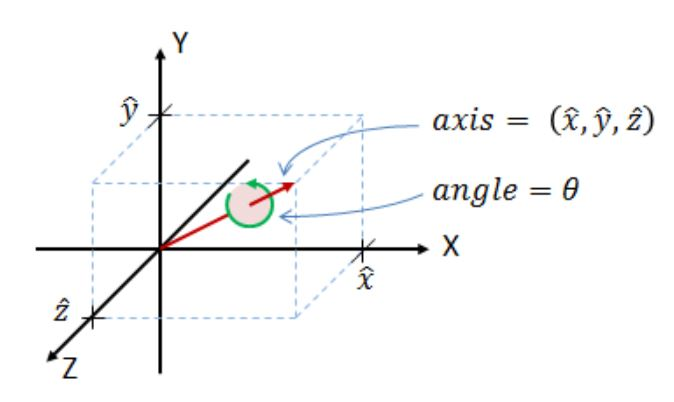
\includegraphics[width=0.7\textwidth]{angleaxis}
	\caption{Angle-axis representation of 3D rotation \cite{quaternionuse}}
	\label{fig:angleaxis}
\end{figure}

Two other concepts are often used to represent the rotation between two coordinate frames: rotation matrices and Euler angles (pitch, roll, yaw). Rotation matrices are useful for rotating 3D points and are discussed in Sections \ref{ssec:2s5s2} and \ref{ssec:2s5s4}. Euler angles are the most common way of describing rotations (particularly in aircraft) due to their simplicity and ease-of-understanding. However, Euler angles depend on a particular sequence of rotations to take place (generally, yaw-pitch-roll, in that order) and are subject to a phenomenon known as “gimbal lock.” In gimbal lock, when the pitch angle of a body reaches ±90°, a singularity occurs in the equations for the Euler angles; the yaw and roll axes become indistinguishable from each other \cite{quaternionuse}. To avoid dealing with this special case, the Madgwick filter uses quaternions to describe rotations between bodies \cite{madgwick}.

Specific uses of quaternions, including rotating a point by a quaternion, rotating a quaternion by another quaternion, and converting between the Euler angle representation and quaternion representation of a rotation can be found in Section \ref{ssec:3s9s1}. For the remainder of this section, quaternions will be used to describe any rotations between coordinate frames.

\subsection{Filter Theory} \label{ssec:4s4s2}
Using an accelerometer, gyroscope, and magnetometer, two different orientation estimates can be formed: one from the relative change in orientation described by gyroscope readings, and one from the absolute measurements of the accelerometer (gives “down” direction) and the magnetometer (gives “magnetic north” direction). For each of these two absolute measurements, two vectors can be defined: one that points towards the true position of the quantity being measured in the global frame (gravity for accelerometer, and magnetic north for magnetometer), and one that points in the direction of the sensor measurement. For example, if the IMU was at a pitch angle of 30° about the y-axis, the vector in Equation \ref{eq:30d} shows true gravity in the global frame and the vector in Equation \ref{eq:30s} shows what the accelerometer would measure (assuming a NED coordinate frame) \cite{madgwick}.

\begin{equation} \label{eq:30d}
	\mathbf{d}= [0, 0, g]
\end{equation}

\begin{equation} \label{eq:30s}
	\mathbf{s}= [-g \cos(30°), 0, g \sin(30°)]
\end{equation}

A minimization problem can be formed for each absolute measurement, where the true vector in the global frame rotated by the current quaternion (orientation estimate of the sensor) should equal the measured vector in the sensor frame. This is represented as an objective function for a single sensor in Equation \ref{eq:1f}, and for the combination of accelerometer and magnetometer in Equation \ref{eq:2f} \cite{madgwick}.

\begin{equation} \label{eq:1f}
	\mathbf{f}({}^S_E\hat{\mathbf{q}}, {}^E\hat{\mathbf{d}}, {}^S\hat{\mathbf{s}}) = {}^S_E\hat{\mathbf{q}}^* \otimes  {}^E\hat{\mathbf{d}} \otimes {}^S_E\hat{\mathbf{q}} - {}^S\hat{\mathbf{s}}
\end{equation}

\begin{equation} \label{eq:2f}
	\mathbf{f}_{g,b}({}^S_E\hat{\mathbf{q}}, {}^S\hat{\mathbf{a}}, {}^E\hat{\mathbf{b}}, {}^S\hat{\mathbf{m}}) = \begin{bmatrix}
		\mathbf{f}_g({}^S_E\hat{\mathbf{q}}, {}^S\hat{\mathbf{a}})\\
		\mathbf{f}_b({}^S_E\hat{\mathbf{q}}, {}^E\hat{\mathbf{b}}, {}^S\hat{\mathbf{m}})
	\end{bmatrix}
\end{equation}

The gradient of the objective function can also be computed; see Equation \ref{eq:1gr} for the general form and Equation \ref{eq:2gr} for the accelerometer / magnetometer combined form. The gradient is defined by the objective function and its Jacobian; the Jacobian of the combined accelerometer / magnetometer objection function can be seen in Equation \ref{eq:jac}. These are used along with the step size \(\mu\) to compute the accelerometer / magnetometer orientation estimate for the next filter update (see Equation \ref{eq:qgr}) \cite{madgwick}.

\begin{equation} \label{eq:1gr}
	\nabla \mathbf{f}({}^S_E\hat{\mathbf{q}}_k, {}^E\hat{\mathbf{d}}, {}^S\hat{\mathbf{s}}) = \mathbf{J}^T({}^S_E\hat{\mathbf{q}}_k, {}^E\hat{\mathbf{d}})\mathbf{f}({}^S_E\hat{\mathbf{q}}_k, {}^E\hat{\mathbf{d}}, {}^S\hat{\mathbf{s}})
\end{equation}

\begin{equation} \label{eq:2gr}
	\nabla \mathbf{f} = \begin{Bmatrix}
		\mathbf{J}_g^T({}^S_E\hat{\mathbf{q}}_{est,t-1})\mathbf{f}_g({}^S_E\hat{\mathbf{q}}_{est,t-1}, {}^S\hat{\mathbf{a}}_t) \\
		\mathbf{J}_{g,b}^T({}^S_E\hat{\mathbf{q}}_{est,t-1}, {}^E\hat{\mathbf{b}}) \mathbf{f}_{g,b}({}^S_E\hat{\mathbf{q}}_{est,t-1}, {}^S\hat{\mathbf{a}}, {}^E\hat{\mathbf{b}}, {}^S\hat{\mathbf{m}})
	\end{Bmatrix}
\end{equation}

\begin{equation} \label{eq:jac}
	\mathbf{J}_{g,b}({}^S_E\hat{\mathbf{q}}, {}^E\hat{\mathbf{b}}) = \begin{bmatrix}
		\mathbf{J}_g^T({}^S_E\hat{\mathbf{q}}) \\
		\mathbf{J}_b^T({}^S_E\hat{\mathbf{q}}, {}^E\hat{\mathbf{b}})
	\end{bmatrix}
\end{equation}

\begin{equation} \label{eq:qgr}
	{}^S_E\mathbf{q}_{\nabla,t} = {}^S_E\hat{\mathbf{q}}_{est,t-1} - \mu_t \frac{\nabla \mathbf{f}}{||\nabla \mathbf{f}||}
\end{equation}

The orientation estimate computed from the gyroscope measurements is described in Equations \ref{eq:gyr} and \ref{eq:gyr2}. This orientation estimate is then combined with the accelerometer / magnetometer orientation estimate in Equation \ref{eq:comb}. The weighting factor \(\gamma_t\) is calculated to ensure the optimal fusion of the two orientation estimates; this calculation is skipped here for brevity \cite{madgwick}.

\begin{equation} \label{eq:gyr}
	{}^S_E\dot{\mathbf{q}}_{\omega,t} = \frac{1}{2} 	{}^S_E\hat{\mathbf{q}}_{est,t-1} \otimes {}^S\boldsymbol{\omega}_t
\end{equation}

\begin{equation} \label{eq:gyr2}
	{}^S_E\mathbf{q}_{\omega,t} = {}^S_E\hat{\mathbf{q}}_{est,t-1} + {}^S_E\dot{\mathbf{q}}_{\omega,t} \Delta t
\end{equation}

\begin{equation} \label{eq:comb}
	{}^S_E\mathbf{q}_{est,t} = \gamma_t {}^S_E\mathbf{q}_{\nabla,t} + (1 - \gamma_t) 	{}^S_E\mathbf{q}_{\omega,t}, \quad 0 \leq \gamma_t \leq 1
\end{equation}

In this algorithm, two errors can be compensated for: magnetic distortion and gyroscope bias drift. Hard iron sources, like permanent magnets in electric motors, can distort the magnetic field around the magnetometer and can be removed with proper calibration (as mentioned in Section \ref{sec:4s3}). Inclination errors, which are the vertical component of soft iron distortions (caused by stray magnetic fields, such as a field generated by running current through a wire), can be compensated for with the Madgwick filter. This is achieved by rotating the magnetometer measurements by the current orientation estimate and using the components of the resulting vector to form the true magnetic north vector. This process is able to remove the vertical effect of soft-iron distortions, but horizontal effects still remain. Equations \ref{eq:mag1} and \ref{eq:mag2} show this process \cite{madgwick}.

\begin{equation} \label{eq:mag1}
	^E\hat{\mathbf{h}}_t = \left[0 \quad h_x \quad h_y \quad h_z\right] = {}^S_E\mathbf{q}_{est,t-1} \otimes {}^S\hat{\mathbf{m}}_t \otimes {}^S_E\mathbf{q}_{est,t-1}^*
\end{equation}

\begin{equation} \label{eq:mag2}
	^E\hat{\mathbf{b}}_t = \left[0 \quad \sqrt{h_x^2 + h_y^2} \quad 0 \quad h_z\right]
\end{equation}

The gyroscope bias drifts over time due to temperature changes and motion. This bias is initially eliminated by calibrating the gyroscope (as mentioned in Section \ref{sec:4s3}), but the Madgwick filter includes a method for removing the drift over time. The drift is estimated using an integral feedback approach: the change in orientation is estimated using the difference between the current and previous orientation estimate, and this estimate is combined with the gyroscope measurements to eliminate the drift over time. Equations \ref{eq:gy1}, \ref{eq:gy2}, and \ref{eq:gy3} show this process \cite{madgwick}.

\begin{equation} \label{eq:gy1}
	{}^S\boldsymbol{\omega}_{\epsilon,t} = 2^S_E\hat{\mathbf{q}}_{est,t-1}^* \otimes {}^S_E\dot{\hat{\mathbf{q}}}_{\epsilon,t}
\end{equation}

\begin{equation} \label{eq:gy2}
	{}^S\boldsymbol{\omega}_{b,t} = \zeta \sum_t {}^S\boldsymbol{\omega}_{\epsilon,t} \Delta t
\end{equation}

\begin{equation} \label{eq:gy3}
	{}^S\boldsymbol{\omega}_{c,t} = {}^S\boldsymbol{\omega}_t - {}^S\boldsymbol{\omega}_{b,t}
\end{equation}

Finally, all of the above concepts are combined to form the Madgwick filter. Figure \ref{fig:madgblock} shows the block diagram for the full system. Some simplifications not covered in this explanation (particularly for the weighting of the two orientation estimates) are implemented into the diagram. Here, two tunable gains are presented: \(\beta\), which is used to modify the weighting factor between the two orientation estimates, and \(\zeta\), which is used to weight the gyroscope bias drift compensation \cite{madgwick}.

\begin{figure}[htbp]
	\centering
	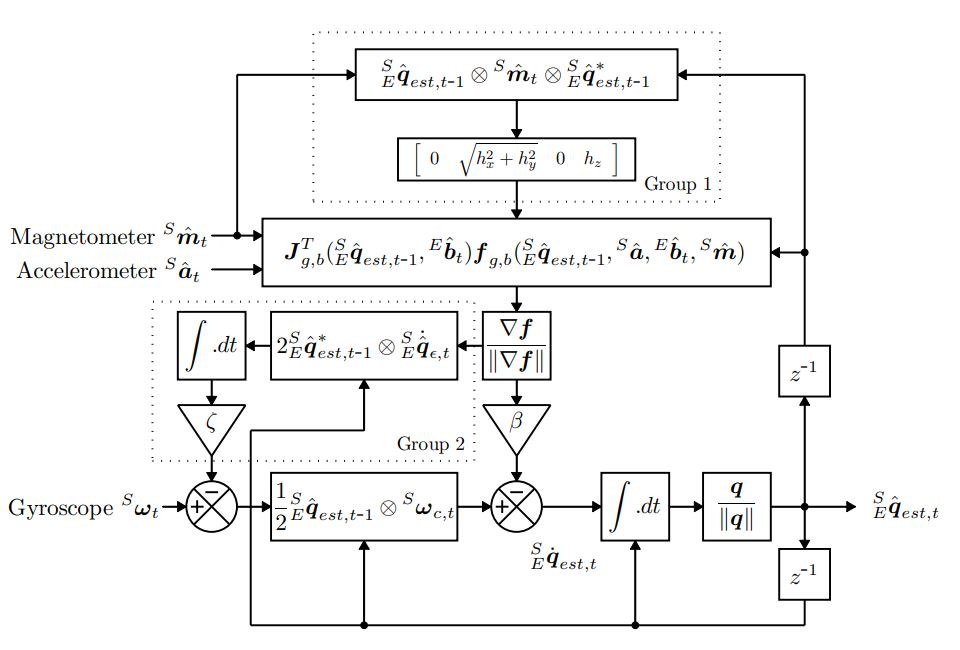
\includegraphics[width=\textwidth]{madgblock}
	\caption{Block diagram for Madgwick filter with accelerometer, gyroscope, and magnetometer (error compensation for magnetic distortion in Group 1 and for gyroscope bias drift in Group 2) \cite{madgwick}}
	\label{fig:madgblock}
\end{figure}

\subsection{Filter Implementation} \label{ssec:4s4s3}
The code implementation of the Madgwick filter used in this thesis is a modified version of Sebastian Madgwick’s C implementation, available on his company’s website \cite{xiotech}. This implementation appears to not incorporate the gyroscope bias drift compensation, and there is no corresponding \(\zeta\) gain used. The code is highly optimized and uses as few scalar arithmetic operations as possible, so some lines may seem fairly complex.

First, the time since the last filter update is calculated using timer TIM13. The timer has a prescalar of 4096 and a period of 65536; it ticks at approximately 67.1kHz and has an overall period of approximately 0.976s. The filter updates based on the update rate of the LSM6DSOX, which is set at 208Hz in this implementation, so there is little worry of exceeding the overall period.

\begin{lstlisting}[language=C++]
timestamp = __HAL_TIM_GET_COUNTER(&htim13);
uint32_t diff_ticks;
if (timestamp >= previousTimestamp) {
	diff_ticks = timestamp - previousTimestamp;
} else {
	diff_ticks = (65536 - previousTimestamp) + timestamp;
}
deltat = (float)diff_ticks * 4096.0f / 275000.0f;
previousTimestamp = __HAL_TIM_GET_COUNTER(&htim13);
\end{lstlisting}

The data from the IMU is then saved in nine floats. The gyroscope readings are converted from degrees per second to radians per second, as required by the filter. The units of the accelerometer and magnetometer do not matter since they are normalized, but they are saved in g’s and Gauss, respectively.

\begin{lstlisting}[language=C++]
float ax = acceleration_g[0];
float ay = acceleration_g[1];
float az = acceleration_g[2];
float gx = angular_rate_dps[0] * 3.14159 / 180.0;
float gy = angular_rate_dps[1] * 3.14159 / 180.0;
float gz = angular_rate_dps[2] * 3.14159 / 180.0;
float mx = magnetic_G[0];
float my = magnetic_G[1];
float mz = magnetic_G[2];
\end{lstlisting}

The rate of change of the quaternion is calculated from the gyroscope data as described in Equation \ref{eq:gyr} \cite{xiotech}.

\begin{lstlisting}[language=C++]
qDot1 = 0.5f * (-q1 * gx - q2 * gy - q3 * gz);
qDot2 = 0.5f * (q0 * gx + q2 * gz - q3 * gy);
qDot3 = 0.5f * (q0 * gy - q1 * gz + q3 * gx);
qDot4 = 0.5f * (q0 * gz + q1 * gy - q2 * gx);
\end{lstlisting}

After this, the accelerometer and magnetometer measurements are normalized. Some auxiliary variables are computed to avoid repeating arithmetic (such as the product of q0 and q1, for example). 

Next, the magnetic distortion calibration described in Equations \ref{eq:mag1} and \ref{eq:mag2} is implemented \cite{xiotech}.

\begin{lstlisting}[language=C++]
hx = mx * q0q0 - _2q0my * q3 + _2q0mz * q2 + mx * q1q1 + _2q1 * my * q2 + _2q1 * mz * q3 - mx * q2q2 - mx * q3q3;
hy = _2q0mx * q3 + my * q0q0 - _2q0mz * q1 + _2q1mx * q2 - my * q1q1 + my * q2q2 + _2q2 * mz * q3 - my * q3q3;
\end{lstlisting}

The gradient descent algorithm steps in Equations \ref{eq:1f} through \ref{eq:qgr} are performed in a highly-optimized manner. These return the computed gradient of the accelerometer / magnetometer quaternion, \(\nabla \mathbf{f}\) \cite{xiotech}.

\begin{lstlisting}[language=C++]
s0 = -_2q2 * (2.0f * q1q3 - _2q0q2 - ax) + _2q1 * ...
s1 = _2q3 * (2.0f * q1q3 - _2q0q2 - ax) + _2q0 * ...	
s2 = -_2q0 * (2.0f * q1q3 - _2q0q2 - ax) + _2q3 * ...
s3 = _2q1 * (2.0f * q1q3 - _2q0q2 - ax) + _2q2 * ...
\end{lstlisting}

The gradient is normalized to give the estimated rate of change of the quaternion. Next, the accelerometer / magnetometer estimate is combined with the estimated rate of change of the quaternion from the gyroscope readings, using \(\beta\) as a weighting factor \cite{xiotech}.

\begin{lstlisting}[language=C++]
qDot1 -= beta * s0;
qDot2 -= beta * s1;
qDot3 -= beta * s2;
qDot4 -= beta * s3;
\end{lstlisting}

Finally, this combined rate of change estimate is integrated using the \verb|deltat| term computed earlier, and is added to the previous orientation estimate quaternion \cite{xiotech}.

\begin{lstlisting}[language=C++]
q0 += qDot1 * deltat / 1000;
q1 += qDot2 * deltat / 1000;
q2 += qDot3 * deltat / 1000;
q3 += qDot4 * deltat / 1000;
\end{lstlisting}

The updated quaternion is then normalized and can be used as the current orientation estimate of the sensor / iSBL array. The filter runs in the background as the STM32 runs the acoustic positioning system code and is paused when recording from the ADC.

\section{Dead-Reckoning} \label{sec:4s5}
Dead reckoning is a ubiquitous and extremely important navigation technique. Before the creation of GPS satellites, it was a primary method for navigating the high seas when celestial navigation was not an option. Similarly, airplane pilots and navigators would use dead reckoning to travel from place to place, taking into account the plane’s relative speed and the velocity of the air around them \cite{britdeadreck}. Hikers and explorers make use of dead reckoning when they use a compass to determine their heading and then walk a certain distance in that direction. Dead reckoning is simply the technique of using time, heading, velocity, and external factors to determine the change in position from a known initial position.

Though GPS and GNSS have drastically changed how the world is navigated, dead reckoning is still commonly used. Submarines that only use GPS for absolute location fixes (as opposed to acoustic positioning methods or similar) often use doppler velocity logs, which measure the velocity of the submarine relative to the ocean floor; when combined with gyromagnetic compass headings, dead reckoning can be used produce a position estimate \cite{surveyurpn}. Pedestrian movements can be estimated using the IMUs in modern smartphones, which allows for position estimation when external sources (WiFi positioning, GPS) are unavailable \cite{sfcomp} \cite{madgstep}. 

Dead reckoning is an inherently error-prone technique: errors in the initial position estimate, speed (or acceleration) measurements, and heading measurements all propagate into future position estimates. To minimize these errors, extremely accurate and calibrated measurement equipment is recommended; for IMUs, Figure \ref{fig:imucomp} in Section \ref{ssec:4s1s1} shows how the performance grade of an IMU correlates to its dead reckoning accuracy. The IMU chosen for this thesis falls between the consumer and industrial performance grades; for this grade, dead reckoning is very inaccurate \cite{imuadvnav}. Despite this limitation, an attempt at dead reckoning using the IMU will be made.

Using IMUs for dead reckoning is inherently more error-prone due to an additional integration requirement. Most dead reckoning methods on ships, submarines, and aircraft use heading and velocity; IMUs measure heading and acceleration. With velocity, only one integration is required to give position, but acceleration requires two. This means that any minuscule error in accelerometer measurements will be propagated into a large position error.

To combat this, a few assumptions are made about the movement of the Fo-SHIP. First, the movement is assumed to be relatively quick - the Fo-SHIP moves from one position to the next in under one second, and then holds that position until another movement is executed. Second, the motion of the Fo-SHIP is not very smooth; the Fo-SHIP interpolates between the initial and final position in discrete steps, and due to the serial nature of the hexapod platforms, any jitter in lower platforms is propagated up to the end effector. As a result, the accelerometer is rarely at rest during movement between set points. Finally, it is assumed that the Fo-SHIP starts at rest and ends at rest; any integrated velocity should start at zero and end at zero, and any non-zero velocity at the end of a move should be considered velocity drift.

These assumptions are quite similar to those made in pedestrian dead reckoning, often known as “gait tracking.” When walking, a pedestrian’s foot starts at rest, moves with large accelerations, and ends at rest. Gait tracking does make use of other assumptions (relatively standardized step sizes among pedestrians, known orientation of the pedestrians’ feet, etc.), but it provides a good starting point for implementing dead reckoning on the Fo-SHIP. For a full underwater implementation, these assumptions would not hold; motion in the water is much more smooth and the underwater vehicle is almost never completely stationary. However, underwater implementations can make use of additional sources of information (doppler velocity logs, input to thrusters, speed of the vehicle relative to the water around it) which are not available in the above-water implementation. For the underwater implementation, making use of these information sources and removing the gait tracking assumptions would be highly encouraged.

The approach taken in this thesis builds off of another Sebastian Madgwick project, “Gait Tracking with x-IMU” \cite{madgstep}. This project is written in Matlab and includes some assumptions not valid for the thesis implementation, so the code has been re-worked significantly. The overall goals and workflow of this implementation are as follows:
\begin{itemize}[noitemsep,topsep=0pt,]
	\item Rotate the accelerometer measurements from the sensor frame to the test frame
	\item Determine if the array is accelerating
	\item Integrate acceleration measurements into a change in velocity
	\item Compensate for velocity drift if the array is stationary
	\item Integrate the current velocity estimate into a change in position
\end{itemize}

First, the accelerometer measurements are rotated from the sensor frame to the test frame. The dead reckoning code runs immediately after the Madgwick filter updates, so the orientation of the sensor frame relative to the test frame is already available. The rotation of the measurements follows the same procedure described in Section \ref{ssec:3s9s1}: rotate the current orientation estimate by the yaw component of the initial orientation to transform from the global frame to the test frame; normalize the quaternion; and then rotate the acceleration measurement vector by the normalized quaternion.

\begin{lstlisting}[language=C++]
// extract the current orientation of the platform
Quaternion quat_raw = {q0, q1, q2, q3};

// create a quaternion to undo initial yaw rotation and apply it to the current quaternion
Quaternion yaw_compensation = create_yaw_quaternion(init_yaw);
Quaternion quat = multiply_quaternions(yaw_compensation,quat_raw);

// normalize the result to ensure it's a valid rotation
normalize_quaternion(&quat);

// rotate the accelerometer readings by the current quaternion to get the acceleration from the sensor frame to the global frame
Point3D acc_temp = {acceleration_g[0], acceleration_g[1], acceleration_g[2]};
Point3D acc_corr_temp = rotatePoint(acc_temp, quat);
\end{lstlisting}

The next step is to determine if the platform is accelerating. As stated above, it is assumed that the platform is moving if the accelerometer readings are significant enough. The absolute value magnitude of the accelerometer readings is calculated and gravity is subtracted from the magnitude to ensure only non-gravitational acceleration is considered.

\begin{lstlisting}[language=C++]
float acc_mag_abs = fabsf(sqrtf(acceleration_g[0]*acceleration_g[0] + acceleration_g[1]*acceleration_g[1] + acceleration_g[2]*acceleration_g[2]) - 1);
\end{lstlisting}

Then, the acceleration magnitude is compared to an experimentally-determined threshold value. MEMS IMUs tend to have fairly noisy measurements, and a stationary sensor may produce a non-zero acceleration magnitude; this threshold ensures that only significant movements are considered. If the acceleration magnitude exceeds the threshold, then the rotated acceleration measurements are integrated into a change in velocity. The \verb|deltat| value is the time since the last Madgwick filter update in milliseconds, as described in Section \ref{ssec:4s4s3}. This thresholding removes considerable drift from the dead reckoning position estimate.

\begin{lstlisting}[language=C++]
if (acc_mag_abs > 0.04){
	// acceleration is in g's, convert to m/s^2
	v_corrected.x -= (acc_corr_temp.x) * deltat/1000 * 9.81; 
	v_corrected.y -= (acc_corr_temp.y) * deltat/1000 * 9.81;
	v_corrected.z -= (acc_corr_temp.z - 1) * deltat/1000 * 9.81;
	acc_stable_cnt = 0;
	acc_stable_flag = 1;
}
\end{lstlisting}

If the threshold is exceeded, then the IMU is considered “non-stable” - it is currently moving relative to the test frame. If it doesn’t exceed the threshold, then it is considered “stable.” If the IMU has been stable for a set number of filter updates after movement is detected (20, in this implementation), then velocity drift compensation is applied. As stated above, another assumption is that if the IMU has been stable for a period of time, it is considered to be stationary; in this case, the velocity should equal zero. This is rarely the case due to velocity drift.

For ease of implementation, the velocity drift is assumed to be some constant bias that adds to each velocity measurement. This bias results in the accumulated velocity ending at some non-zero value when the IMU becomes stable after moving. Figure \ref{fig:veldrift} provides a visualization of this phenomenon, with the line representing \verb|v_corrected[]| over time.

\begin{figure}[htbp]
	\centering
	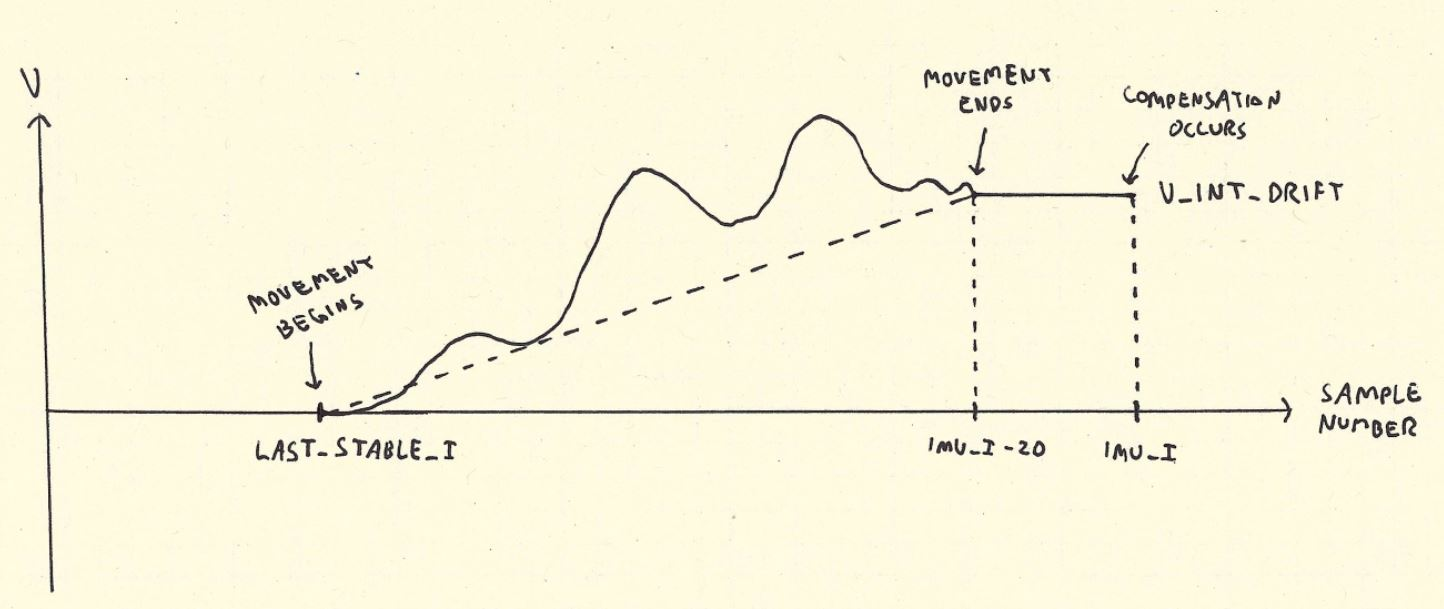
\includegraphics[width=\textwidth]{veldrift}
	\caption{IMU velocity drift example, 1D case}
	\label{fig:veldrift}
\end{figure}

The change in position can be described as the area underneath this velocity curve (or the integration over time). This constant velocity drift can be removed from the change in position by subtracting the area of two regions on the graph: the triangular region during the time of motion, and the rectangular region when the IMU is stationary. This is only possible because the current velocity of the IMU is integrated into a change in position at every time step, as seen at the end of this section.

First, the value of \verb|v_int_drift[]| is calculated as the difference between the initial velocity and the final velocity. For this implementation, the initial velocity will always be zero - however, a vector \verb|v_corrected_last_stable[]| is used to represent the initial velocity in case this implementation is modified.

\begin{lstlisting}[language=C++]
Point3D v_int_drift;
v_int_drift.x = v_corrected.x - v_corrected_last_stable.x;
v_int_drift.y = v_corrected.y - v_corrected_last_stable.y;
v_int_drift.z = v_corrected.z - v_corrected_last_stable.z;
\end{lstlisting}

Next, the time between the start and end of motion is calculated. \verb|imu_i| is a counter that tracks how many filter updates have occurred (and overflows at 10,000 iterations), and \verb|last_stable_i| saves the index of when the IMU started to move. \verb|imu_diff| is the number of filter updates between the start of movement and the end of movement of the IMU (the width of the triangle in Figure \ref{fig:veldrift}).

\begin{lstlisting}[language=C++]
float i_diff = (imu_i > last_stable_i) ? (float) imu_i - last_stable_i : (float) 10000 - last_stable_i + imu_i;
i_diff += 1;
i_diff -= (float) acc_stable_cnt;
\end{lstlisting}

Next, the area of the two regions is subtracted from the current change-in-position estimate. Since \verb|deltat| can fluctuate,  the update rate of the LSM6DSOX (208Hz) is used to convert the sample count to time. This is a simplification, and summing the values of \verb|deltat| for each iteration that the IMU is moving would give a more precise result.

\begin{lstlisting}[language=C++]
delta_x_imu.x -= (v_int_drift.x * ((i_diff / 2) + (float)acc_stable_cnt) / sampleFreq);
delta_x_imu.y -= (v_int_drift.y * ((i_diff / 2) + (float)acc_stable_cnt) / sampleFreq);
delta_x_imu.z -= (v_int_drift.z * ((i_diff / 2) + (float)acc_stable_cnt) / sampleFreq);
\end{lstlisting}

Finally, the velocity drift value is subtracted from the current velocity estimate. This always resets \verb|v_corrected[]| to the value of the last stable velocity \verb|v_corrected_last_stable[]|, which in practice is always zero. A flag, \verb|acc_stable_flag|, is used to ensure that the velocity drift compensation only occurs once for every chunk of movement; here, it is reset to zero.

\begin{lstlisting}[language=C++]
v_corrected.x -= v_int_drift.x;
v_corrected.y -= v_int_drift.y;
v_corrected.z -= v_int_drift.z;
acc_stable_flag = 0;  // until the system is unstable again, don't re-account for velocity drift
\end{lstlisting}

If the IMU is stable and the velocity drift compensation has already been applied, then the \verb|last_stable_i| is updated to the current \verb|imu_i| value. Additionally, the last stable velocity is set to the current velocity (always zero in this implementation).

\begin{lstlisting}[language=C++]
else if (!acc_stable_flag){
	last_stable_i = imu_i;
	v_corrected_last_stable.x = v_corrected.x;
	v_corrected_last_stable.y = v_corrected.y;
	v_corrected_last_stable.z = v_corrected.z;
}
\end{lstlisting}

Lastly, for every filter update (does not matter if the IMU is stable or moving), the change in position is updated using the current velocity of the IMU. This is the second integration step that occurs, following the first integration of acceleration to velocity in the beginning of the code.

\begin{lstlisting}[language=C++]
delta_x_imu.x += v_corrected.x * deltat/1000;
delta_x_imu.y += v_corrected.y * deltat/1000;
delta_x_imu.z += v_corrected.z * deltat/1000;
\end{lstlisting}

The vectors for the change in position, corrected velocity, and last stable velocity, as well as the counters \verb|imu_i| and \verb|last_stable_i|, are reset after a complete acoustic position estimate. The values are all set to zero after the STM32 sends its position estimate data to the ESP32 and Fo-SHIP.

\begin{lstlisting}[language=C++]
v_corrected.x = 0;
v_corrected.y = 0;
v_corrected.z = 0;
delta_x_imu.x = 0;
delta_x_imu.y = 0;
delta_x_imu.z = 0;
v_corrected_last_stable.x = 0;
v_corrected_last_stable.y = 0;
v_corrected_last_stable.z = 0;
imu_i = 0;
last_stable_i = 0;
\end{lstlisting}

The result of the dead reckoning is the change in position since the last acoustic position estimate, and it is stored in \verb|delta_x_imu[]|. This relative change in position is fed into a Kalman filter along with the absolute acoustic position estimate. Section \ref{sec:5s4} details how this is accomplished.

\section{System Validation} \label{sec:4s6}
After being implemented in code, both the orientation estimation system (the Madgwick filter) and the dead reckoning system were tested and validated to ensure accuracy. The Madgwick filter implementation has one gain, \verb|beta|, that must be tuned. Higher values of \verb|beta| imply more trust in the accelerometer and magnetometer measurements, and tend to lead to faster convergence (and less time delay when quick movements take place).

A variety of tests were run with different \verb|beta| values and select results are detailed below. The Fo-SHIP was moved to different set points and the orientation was measured over time using Euler angle representation (converted from the Madgwick filter output quaternion). For future testing, it would be recommended to save and plot the set points in the same graph as the orientation estimate results to better verify the accuracy of the filter.

For Figures \ref{fig:1b3} through \ref{fig:1b05}, the Fo-SHIP followed this list of instructions:
\begin{itemize}[noitemsep,topsep=0pt,]
	\item Start at zero for all axes
	\item Move to roll = 24° over 1.2 seconds
	\item Hold position for 0.8 seconds
	\item Move to roll = 0° over 1.2 seconds
	\item Hold position for 0.8 seconds
	\item Move to pitch = 24° over 1.2 seconds
	\item Hold position for 0.8 seconds
	\item Move to pitch = 0° over 1.2 seconds
\end{itemize}

Values of \verb|beta| above 0.1 produced very noisy results, and a value of 0.05 produced significant drift over time. This is expected: large values of \verb|beta| place lots of trust in the accelerometer and magnetometer measurements, which are very noisy when moving; and small values place more trust in the gyroscope measurements, which have non-zero noise when stationary that produces drift over time. Drift in the yaw axis was minimal for large \verb|beta| values and significant for small values.

\begin{figure}[htbp]
	\centering
	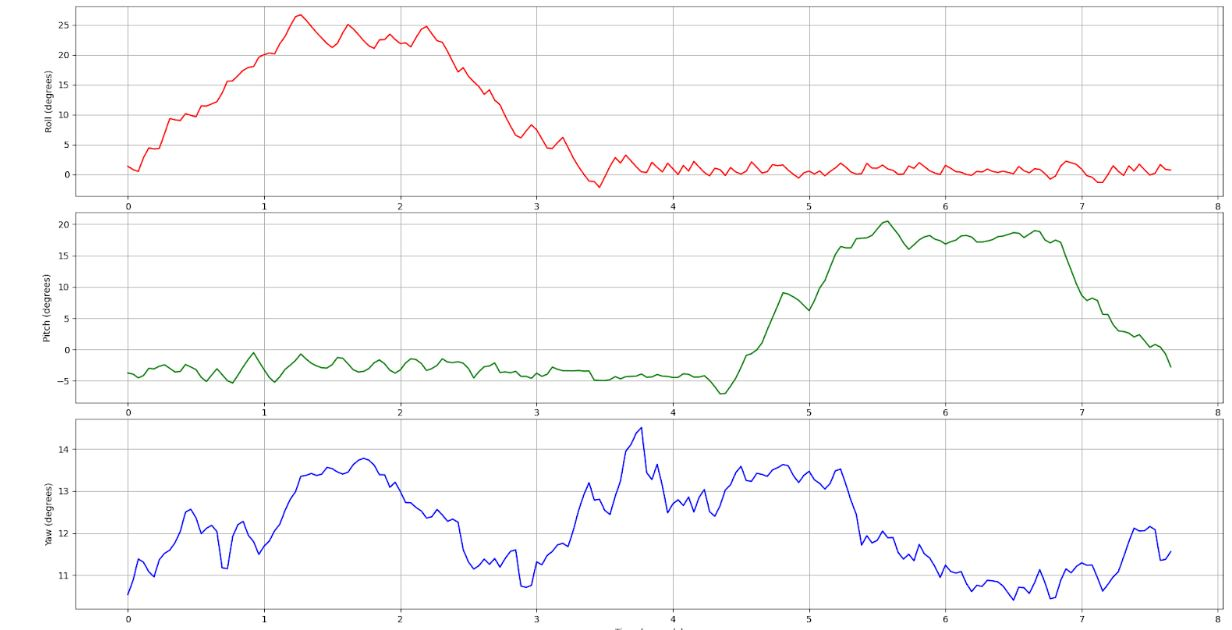
\includegraphics[width=\textwidth]{1b3}
	\caption{\texttt{beta = 0.3}, roll and pitch test with holds between}
	\label{fig:1b3}
\end{figure}

\begin{figure}[htbp]
	\centering
	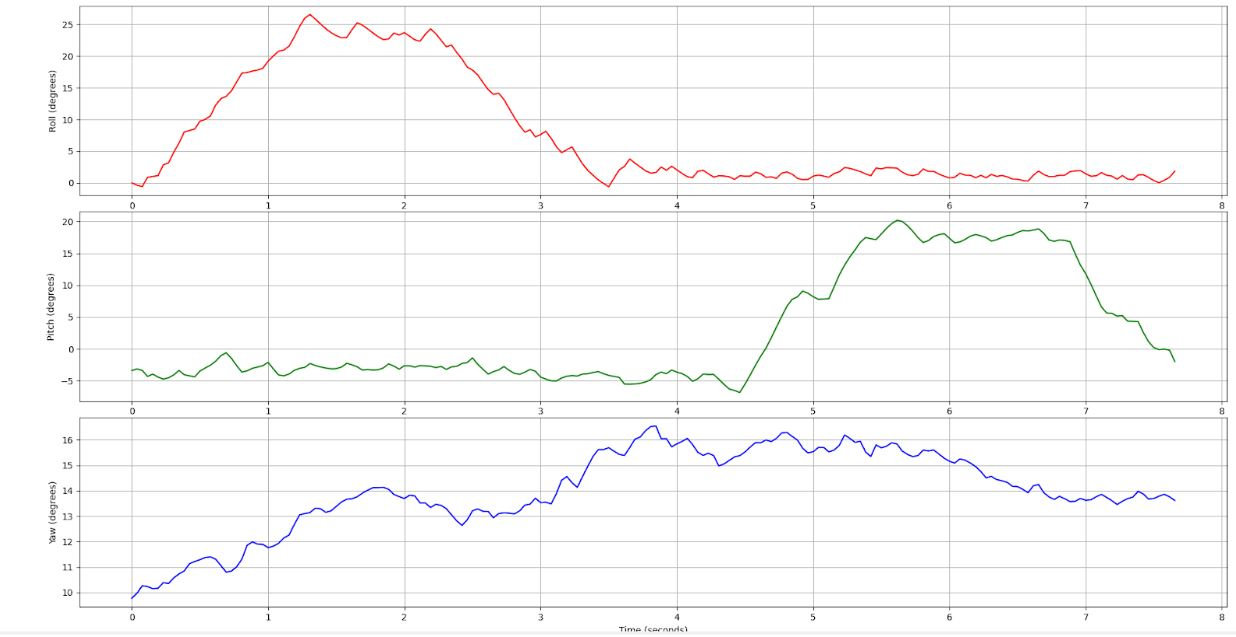
\includegraphics[width=\textwidth]{1b2}
	\caption{\texttt{beta = 0.2}, roll and pitch test with holds between}
	\label{fig:1b2}
\end{figure}

\begin{figure}[htbp]
	\centering
	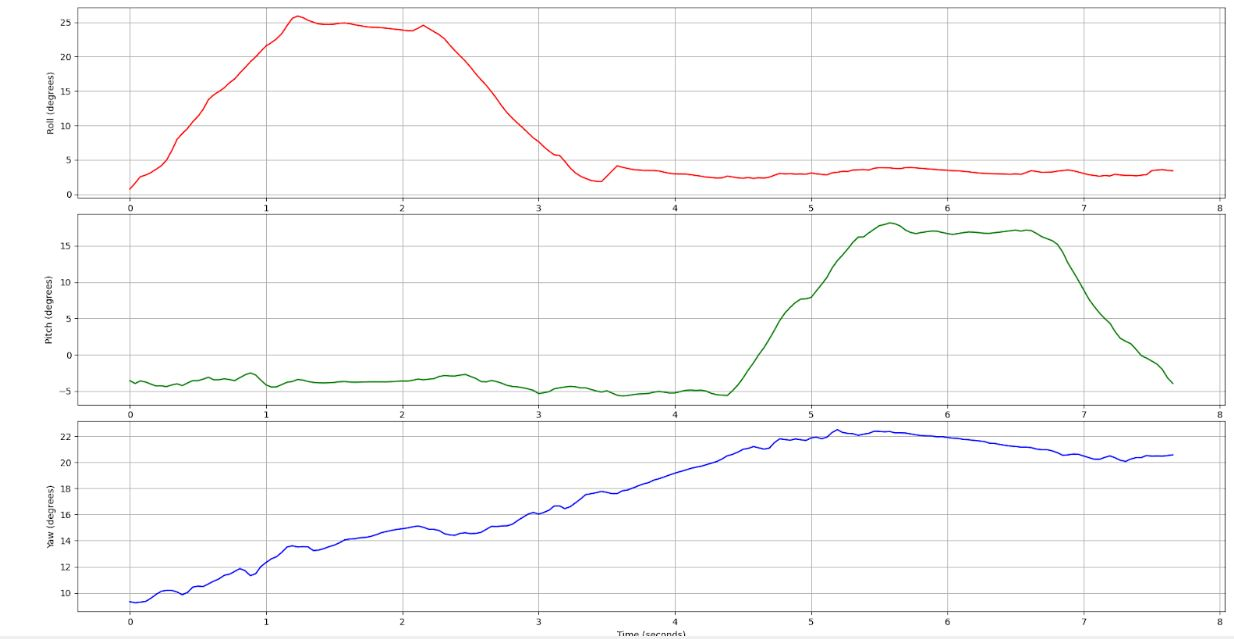
\includegraphics[width=\textwidth]{1b1}
	\caption{\texttt{beta = 0.1}, roll and pitch test with holds between}
	\label{fig:1b1}
\end{figure}

\begin{figure}[htbp]
	\centering
	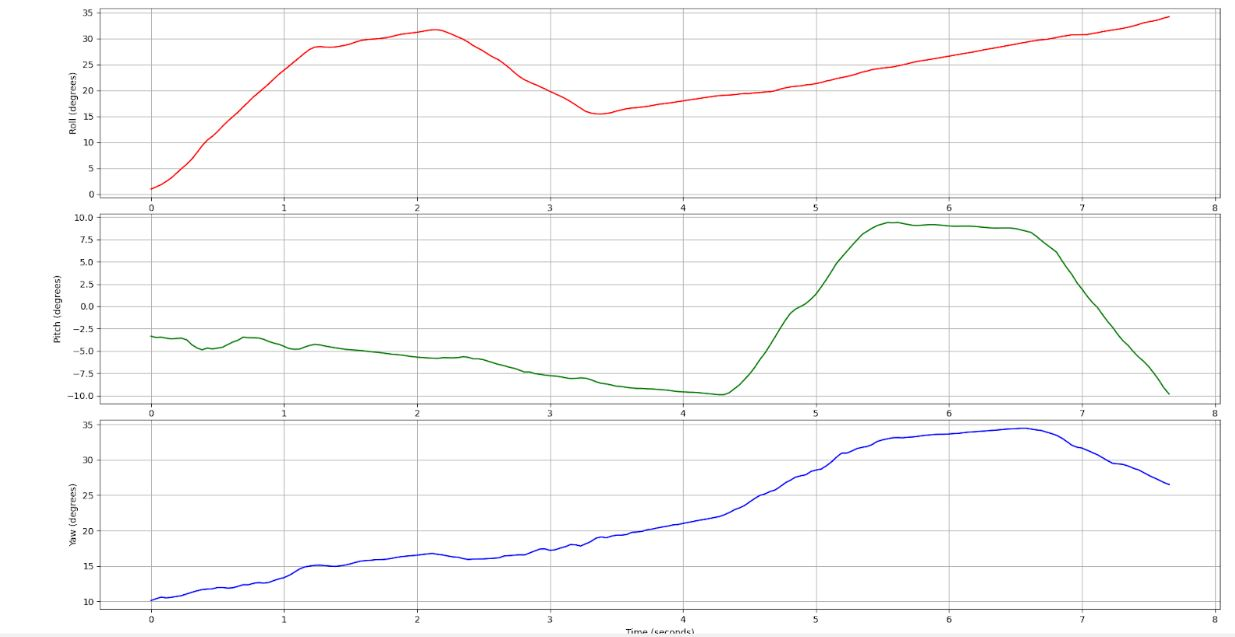
\includegraphics[width=\textwidth]{1b05}
	\caption{\texttt{beta = 0.05}, roll and pitch test with holds between}
	\label{fig:1b05}
\end{figure}

\pagebreak

Due to the poor results of \verb|beta = 0.3|, further tests were not run with this value. For Figures \ref{fig:2b2} through \ref{fig:2b05}, the Fo-SHIP followed these movements:
\begin{itemize}[noitemsep,topsep=0pt,]
	\item Start at zero for all axes
	\item Move to roll = 45° over 0.8 seconds
	\item Move to roll = -45° over 1.6 seconds
	\item Move to roll = 0° over 0.8 seconds
	\item Move to pitch = 45° over 0.8 seconds
	\item Move to pitch = -45° over 1.6 seconds
	\item Move to pitch = 0° over 0.8 seconds
\end{itemize}

The results of this test were much better than the previous test. The higher value of \verb|beta| still produce noisier estimates for all angles, and the lower value still contained significant drift. The yaw values are positively correlated with the pitch values due to initial misalignment of the Fo-SHIP; if it were properly aligned with yaw = 0°, the yaw values would be much more constant.

\begin{figure}[htbp]
	\centering
	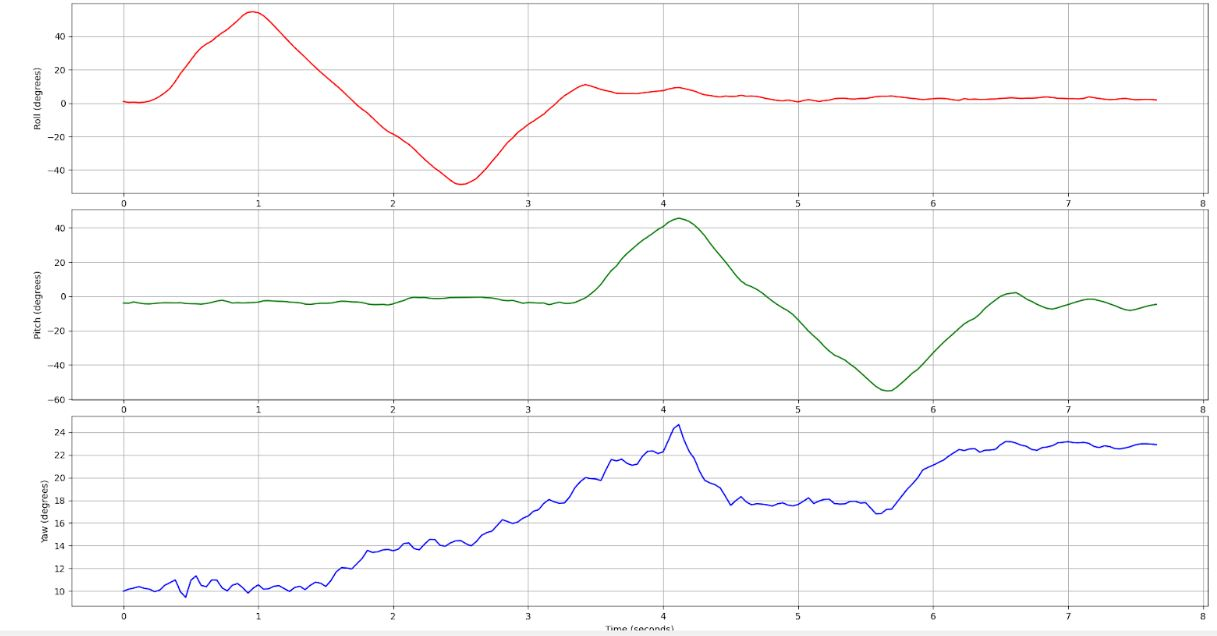
\includegraphics[width=\textwidth]{2b2}
	\caption{\texttt{beta = 0.2}, roll and pitch test with no holds}
	\label{fig:2b2}
\end{figure}

\begin{figure}[htbp]
	\centering
	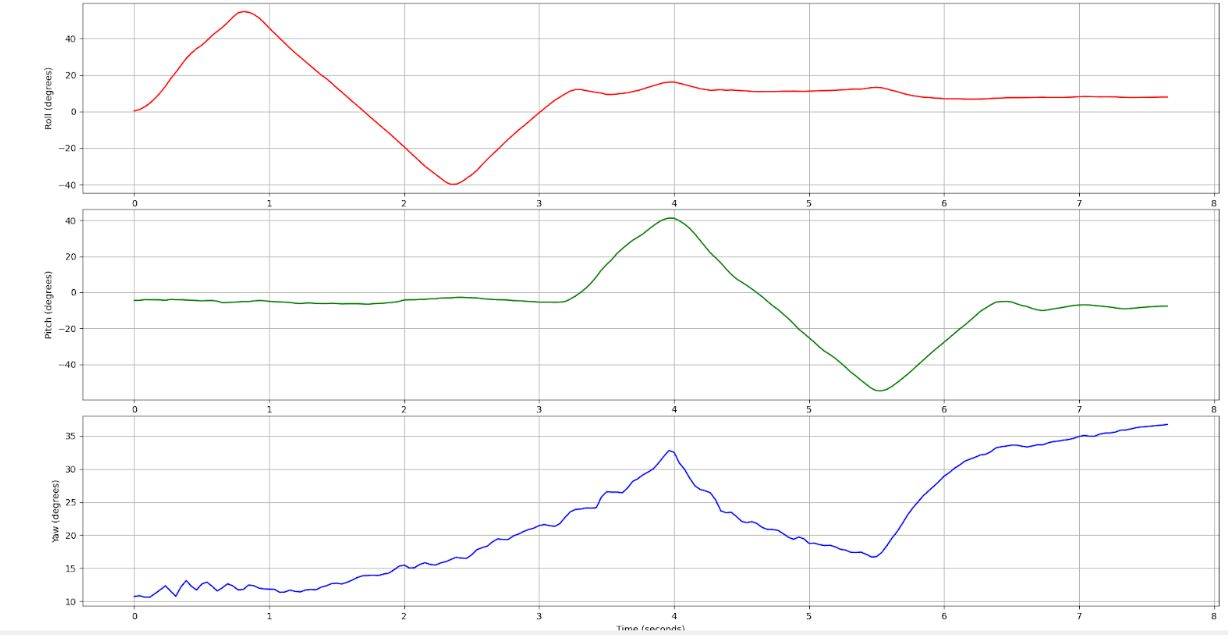
\includegraphics[width=\textwidth]{2b1}
	\caption{\texttt{beta = 0.1}, roll and pitch test with no holds}
	\label{fig:2b1}
\end{figure}

\begin{figure}[htbp]
	\centering
	\includegraphics[width=\textwidth]{2b5}
	\caption{\texttt{beta = 0.05}, roll and pitch test with no holds}
	\label{fig:2b05}
\end{figure}

Note that the yaw component tends to be the least accurate across all the tests performed. This is to be expected; the magnetometer (which provides the absolute reference for yaw) is subject to many external magnetic fields (24 servo motors pulling up to five amps of current, power and data lines from the iSBL receivers placed near the IMU, etc.). Even when stationary, the Earth’s magnetic field is quite weak compared to the non-moving electronics near the IMU.

\pagebreak

The value of \verb|beta = 0.1| produced the least noisy orientation estimate over both tests while not drifting, so it was chosen as the starting point for the optimal \verb|beta| value. After much tuning and testing, the value of \verb|beta = 0.11| was found to give the best orientation estimate with the current implementation of the Madgwick filter. Figure \ref{fig:1b11} shows the results of a test where the maximum range of the Fo-SHIP was used: roll = ±60°, pitch = ±60°, and yaw = ±16°.

\begin{figure}[htbp]
	\centering
	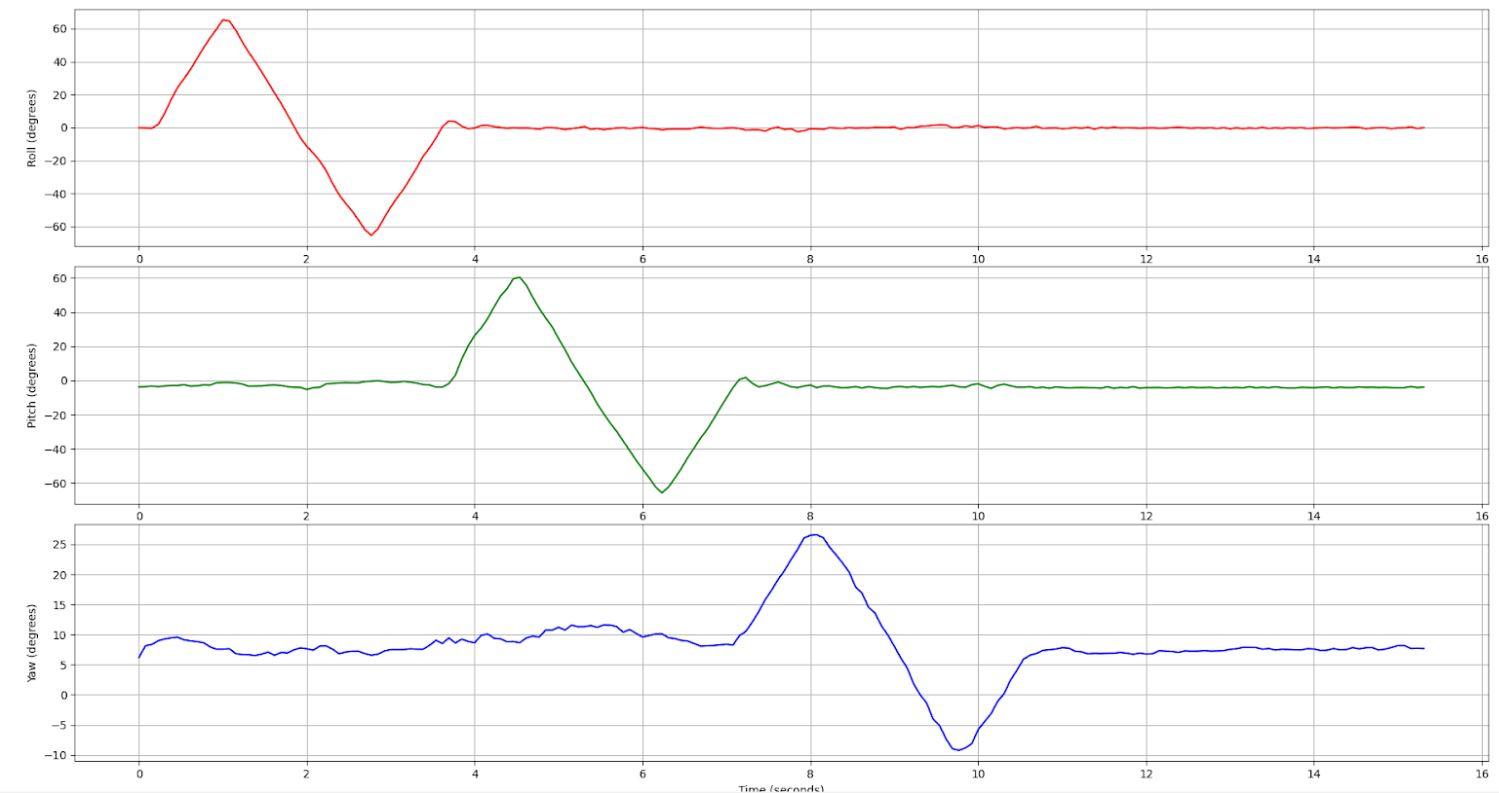
\includegraphics[width=\textwidth]{1b11}
	\caption{\texttt{beta = 0.11}, full Fo-SHIP range-of-motion test}
	\label{fig:1b11}
\end{figure}

Through these tests (and referencing similar implementations of sensor fusion filters running on consumer-grade IMUs \cite{madgwick} \cite{sfcomp} \cite{ekfmadmah} \cite{xiotech}), the steady-state accuracy of the orientation estimate was estimated for each axis of rotation; the results are shown below in Table \ref{tab:angleacc}. Note that this only holds for stationary orientation estimates; the accuracy of the orientation estimate during dynamic movement cannot be easily computed, and is estimated to be at least twice as worse as the steady-state accuracy. Also, note that the accuracies in Table \ref{tab:angleacc} are only estimates. The Fo-SHIP does not have the positional accuracy to properly validate these numbers, and they were estimated using results from similar implementations as well as a few steady-state tests.

\begin{table}[htbp]
	\centering
	\caption{Estimated accuracy of Madgwick filter orientation estimate}
	\label{tab:angleacc}
	\begin{tabular}{|c|c|}
		\hline
		Euler angle representation & Estimated accuracy \\
		\hline
		Roll (about x-axis) & ±1° \\
		\hline
		Pitch (about y-axis) & ±1° \\
		\hline
		Yaw (about z-axis) & ±2° \\
		\hline
	\end{tabular}
\end{table}

The dead reckoning position estimate was often off by a significant factor. The change in position given by the dead reckoning approach is fairly complex and has many sources of error:
\begin{itemize}[noitemsep,topsep=0pt,]
	\item Incorrect orientation estimate (especially when moving) can result in incorrectly rotated acceleration vectors
	\item Small accelerations below the threshold were not incorporated into the motion of the platform
	\item Acceleration errors propagate twice through the position estimate (double integration)
	\item The constant velocity drift bias may be an oversimplification for the true velocity drift bias
	\item The update rate of the Madgwick filter (and the accelerometer) are relatively low compared to other dead reckoning systems \cite{imuadvnav} \cite{ekfmadmah}
\end{itemize}

Table \ref{tab:dracc} shows some position estimates computed by the dead reckoning algorithm for z-axis movements only. The estimated change in position tends to be in the correct direction, but often undershoots the true magnitude of the movement. This is to be expected, given the assumptions made for the algorithm (see Section \ref{sec:4s5}) and the sources of error above.

\begin{table}[htbp]
	\centering
	\caption{True and estimated changes in position using dead reckoning}
	\label{tab:dracc}
	\renewcommand{\arraystretch}{1.2}
	\begin{tabular}{|c|c|c|c|c|c|}
		\hline
		\multicolumn{3}{|c|}{\textbf{\begin{tabular}[c]{@{}c@{}}True Change in\\Position, mm\\(Fo-SHIP)\end{tabular}}} & 
		\multicolumn{3}{c|}{\textbf{\begin{tabular}[c]{@{}c@{}}Estimated Change in\\Position, mm\\(Dead Reckoning)\end{tabular}}} \\
		\hline
		\rule{0pt}{4ex}
		x & y & z & x & y & z \\[2ex]
		\hline
		0 & 0 & 10 & 2.1 & 0 & 6.3 \\
		\hline
		0 & 0 & 10 & 4.2 & 0.3 & 7.4 \\
		\hline
		0 & 0 & 10 & 2.9 & -0.9 & 5 \\
		\hline
		0 & 0 & -10 & 0.8 & 0.2 & -5.2 \\
		\hline
		0 & 0 & -10 & -1 & 0.3 & -8.6 \\
		\hline
		0 & 0 & -10 & -2.7 & 0.8 & -7.9 \\
		\hline
		0 & 0 & 30 & 6 & 0.6 & 20.1 \\
		\hline
		0 & 0 & 30 & -4.2 & 1.1 & 15.7 \\
		\hline
		0 & 0 & 30 & 1.3 & 0 & 22.5 \\
		\hline
		0 & 0 & -30 & 2 & -0.7 & -10 \\
		\hline
		0 & 0 & -30 & 3.5 & 1.2 & -26.3 \\
		\hline
		0 & 0 & -30 & -2.1 & -2.5 & -20.5 \\
		\hline
	\end{tabular}
\end{table}

Despite this inaccuracy, the dead reckoning measurements can give good insight into the motion of the iSBL array. When the array is stationary for multiple acoustic position estimates, the change in position given by the dead reckoning algorithm is zero; when it is moving between estimates, the change in position given is non-zero. This helps inform the Kalman filter model about the relative motion of the system and can result in better position estimates than the acoustic position estimate alone. The results and impact of the dead reckoning algorithm on the position estimate of the system are discussed in Chapter \ref{chap:6c}.

\bibliographystyle{IEEEtran}
\bibliography{../thesis}

\end{document}